\chapter{\ifproject%
\ifenglish Project Structure and Methodology\else โครงสร้างและขั้นตอนการทำงาน\fi
\else%
\ifenglish Project Structure\else โครงสร้างของโครงงาน\fi
\fi
}

ในบทนี้จะกล่าวถึงหลักการ, การนำทฤษฎีที่เกี่ยวข้องมาประยุกต์ใช้ และการออกแบบของระบบ

\makeatletter

% \renewcommand\section{\@startsection {section}{1}{\z@}%
%                                    {13.5ex \@plus -1ex \@minus -.2ex}%
%                                    {2.3ex \@plus.2ex}%
%                                    {\normalfont\large\bfseries}}

\makeatother
%\vspace{2ex}
% \titleformat{\section}{\normalfont\bfseries}{\thesection}{1em}{}
% \titlespacing*{\section}{0pt}{10ex}{0pt}

\section{การจัดเก็บข้อมูล}
โดยข้อมูลราคาหุ้นทุกตัวจะมีแหล่งที่มาจาก 2 ที่ก็คือ AlphaVantage และ Finnhub โดย AlphaVantage จะให้ข้อมูลย้อนหลังไป 2 ปี ส่วน Finnhub จะเอาไว้ใช้อัพเดท
ข้อมูลแบบ real-time ทุกๆ 1 ชม. เราใช้ MongoDB เป็น Database สำหรับจัดเก็บข้อมูลตลาดหุ้น และตัวชี้วัดทางเทคนิคที่เราต้องการใช้ เช่น RSI, MA เป็นต้น

ในตอนเริ่มตันนั้นเราดึงข้อมูลที่ต้องการมาจาก AlphaVantage ซึ่งก็คือข้อมูลตลาดหุ้นย้อนหลัง 2 ปีโดยใช้ API ของ AlphaVantage 
และเก็บข้อมูลลง MongoDB ด้วย Rust โดยมีการแปลงข้อมูลให้เป็นในรูปแบบข้อมูลตลาดของเราซึ่งก็จะประกอบด้วย
\begin{enumerate}
    \item ticker
    \item open
    \item close
    \item high
    \item low
    \item volume
\end{enumerate}


\begin{figure}[ht]
    \centering
    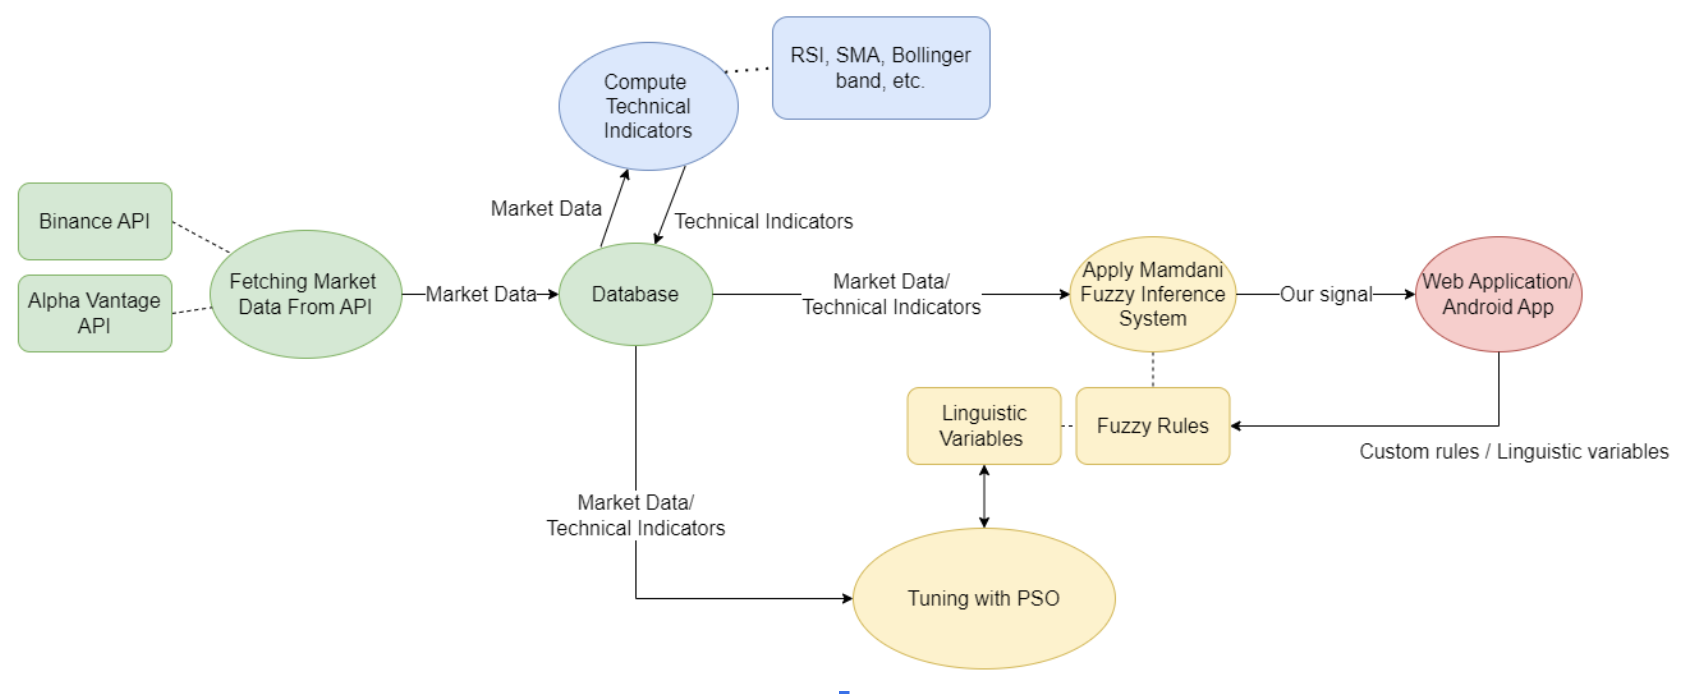
\includegraphics[width=\textwidth]{images/overview.png}
    \caption{โครงสร้างของโครงงาน}
    \label{fig:1}
\end{figure}